\chapter{$f$-Divergences and their Variational Bounds}
\label{ch:f_divergence}

% 1. Descriptive Opening
In the journey to build machines that can generate complex data---from photorealistic images to coherent human language---a central challenge emerges: how do we measure the distance between the distribution of data our model generates and the true distribution of the world? If we can quantify this discrepancy, we can minimize it. We previously encountered the Kullback-Leibler (KL) divergence, a fundamental measure of relative entropy. However, the KL divergence is just one lens through which to view the difference between distributions. Depending on the nature of the data and the goals of the model, we may want to penalize different types of errors. Should the model cover all modes of the true distribution (mode-covering), even at the risk of generating unrealistic samples? Or should it focus on a single mode (mode-seeking) to ensure high-fidelity outputs, even if it ignores other parts of the data space?

This need for a flexible, parameterized family of statistical distances leads us to the concept of $f$-divergences, introduced independently by Csisz\'{a}r (1967) and Ali and Silvey (1966). An $f$-divergence generalizes the KL divergence by defining the distance between two probability distributions $P$ and $Q$ using a convex function $f$. By choosing different functions for $f$, we recover a wide array of well-known divergences, including the Total Variation distance, the Hellinger distance, the Pearson $\chi^2$ divergence, and the Jensen-Shannon divergence. Each of these distances imposes a distinct geometric structure on the space of probability distributions, dictating how a generative model will behave when optimized to minimize that distance.

However, a significant practical hurdle remains. In the context of deep learning, we rarely have access to the exact probability density functions $P$ and $Q$. Instead, we only have empirical access to samples drawn from these distributions: a dataset $\mathcal{D} \sim P_{\text{data}}$ and a batch of generated samples from $p_\theta(x|z)$. The standard definition of an $f$-divergence involves an integral over the probability densities, which is typically intractable to compute directly in high-dimensional spaces. 

To bridge the gap between the elegant theory of $f$-divergences and the empirical reality of deep learning, we turn to convex analysis, specifically the concept of Fenchel conjugacy. By expressing the convex function $f$ in terms of its convex conjugate $f^*$, we can reformulate the intractable integral of the $f$-divergence into a tractable optimization problem over a family of functions. This mathematical maneuver, heavily popularized in deep learning by the $f$-GAN framework (Nowozin et al., 2016) and the Nguyen-Wainwright-Jordan (NWJ) estimator, transforms the problem of density estimation into a problem of binary classification or density ratio estimation. It provides the theoretical bedrock for understanding why and how adversarial networks---where a discriminator network effectively learns to approximate this variational bound---actually work.

In this chapter, we will rigorously define the family of $f$-divergences, explore their key mathematical properties, and derive their variational bounds. We will see how this variational perspective allows us to estimate these divergences purely from samples, unlocking a unified framework for training generative models.

% 2. Mathematical Core
\section{The Geometry of $f$-Divergences}

Let $P$ and $Q$ be two probability distributions defined over a common measurable space $\mathcal{X}$, such that $P$ is absolutely continuous with respect to $Q$ (denoted $P \ll Q$). This absolute continuity ensures that the Radon-Nikodym derivative, or density ratio, $dP/dQ$ exists. For continuous distributions with probability density functions $p(x)$ and $q(x)$, this ratio is simply $p(x)/q(x)$.

\begin{definition}[$f$-Divergence]
Let $f: (0, \infty) \to \mathbb{R}$ be a convex function such that $f(1) = 0$. Furthermore, suppose $f$ is strictly convex at $1$. The $f$-divergence from distribution $P$ to distribution $Q$ is defined as:
\begin{equation}
    D_f(P \parallel Q) = \int_{\mathcal{X}} q(x) f\left( \frac{p(x)}{q(x)} \right) dx = \mathbb{E}_{x \sim Q} \left[ f\left( \frac{p(x)}{q(x)} \right) \right].
\end{equation}
\end{definition}

The condition $f(1) = 0$ ensures that the divergence between a distribution and itself is zero, $D_f(P \parallel P) = 0$. The convexity of $f$ guarantees that the divergence is non-negative.

\begin{theorem}[Non-negativity of $f$-Divergence]
For any two distributions $P$ and $Q$, and any convex function $f$ with $f(1)=0$, $D_f(P \parallel Q) \ge 0$.
\end{theorem}
\begin{proof}
This is a direct application of Jensen's inequality. Since $f$ is a convex function, we can bring the expectation outside the function:
\begin{align*}
    D_f(P \parallel Q) &= \mathbb{E}_{x \sim Q} \left[ f\left( \frac{p(x)}{q(x)} \right) \right] \\
                       &\ge f\left( \mathbb{E}_{x \sim Q} \left[ \frac{p(x)}{q(x)} \right] \right) \\
                       &= f\left( \int_{\mathcal{X}} q(x) \frac{p(x)}{q(x)} dx \right) \\
                       &= f\left( \int_{\mathcal{X}} p(x) dx \right) \\
                       &= f(1) = 0.
\end{align*}
Equality holds if and only if $p(x) = q(x)$ almost everywhere, provided $f$ is strictly convex around $1$.
\end{proof}

\subsection{A Zoo of Divergences}
By selecting different generator functions $f(u)$, we can instantiate a variety of well-known distance measures. Here we list a few prominent examples:

\begin{itemize}
    \item \textbf{Kullback-Leibler (KL) Divergence}: Let $f(u) = u \log u$. Then $D_f(P \parallel Q) = \int q(x) \frac{p(x)}{q(x)} \log \frac{p(x)}{q(x)} dx = D_{\text{KL}}(P \parallel Q)$.
    \item \textbf{Reverse KL Divergence}: Let $f(u) = -\log u$. Then $D_f(P \parallel Q) = \int q(x) \left(-\log \frac{p(x)}{q(x)}\right) dx = D_{\text{KL}}(Q \parallel P)$.
    \item \textbf{Pearson $\chi^2$ Divergence}: Let $f(u) = (u-1)^2$. Then $D_f(P \parallel Q) = \int q(x) \left(\frac{p(x)}{q(x)} - 1\right)^2 dx = \int \frac{(p(x)-q(x))^2}{q(x)} dx$.
    \item \textbf{Total Variation Distance}: Let $f(u) = \frac{1}{2}|u-1|$. Then $D_f(P \parallel Q) = \frac{1}{2} \int q(x) \left|\frac{p(x)}{q(x)} - 1\right| dx = \frac{1}{2} \int |p(x) - q(x)| dx$.
    \item \textbf{Jensen-Shannon (JS) Divergence}: Let $f(u) = -(u+1)\log\frac{u+1}{2} + u\log u$. This leads to a symmetrized divergence bounded between $0$ and $\log 2$.
\end{itemize}

% TikZ Figure 1: Plotting generator functions f(u)
\begin{figure}[htbp]
\centering
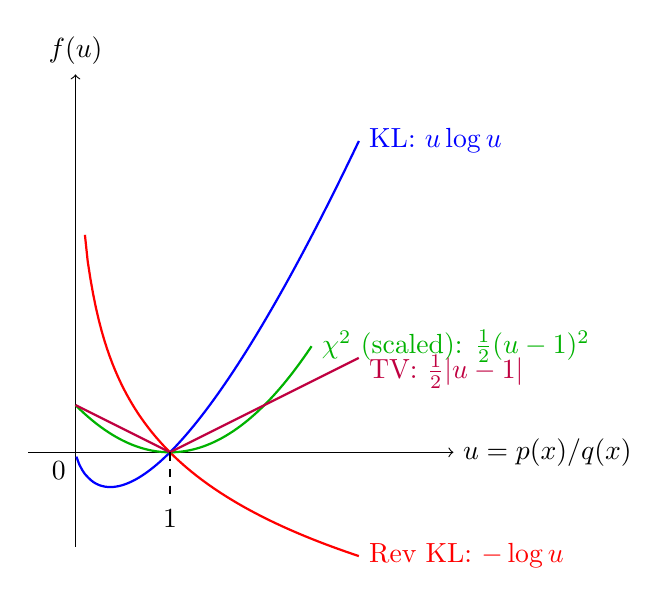
\begin{tikzpicture}[scale=1.2]
    \draw[->] (-0.5,0) -- (4,0) node[right] {$u = p(x)/q(x)$};
    \draw[->] (0,-1) -- (0,4) node[above] {$f(u)$};
    
    % u log u (KL)
    \draw[thick, blue, domain=0.01:3, samples=100] plot (\x, {\x*ln(\x)}) node[right] {KL: $u \log u$};
    
    % -log u (Rev KL)
    \draw[thick, red, domain=0.1:3, samples=100] plot (\x, {-ln(\x)}) node[right] {Rev KL: $-\log u$};
    
    % (u-1)^2 (Pearson chi^2) - scale down a bit for visibility
    \draw[thick, green!70!black, domain=0:2.5, samples=100] plot (\x, {0.5*(\x-1)*(\x-1)}) node[right] {$\chi^2$ (scaled): $\frac{1}{2}(u-1)^2$};
    
    % 0.5|u-1| (Total Variation)
    \draw[thick, purple, domain=0:3, samples=100] plot (\x, {0.5*abs(\x-1)}) node[right, yshift=-5pt] {TV: $\frac{1}{2}|u-1|$};
    
    \draw[dashed] (1,0) -- (1,-0.5) node[below] {$1$};
    \node[below left] at (0,0) {$0$};
\end{tikzpicture}
\caption{Various generator functions $f(u)$ for $f$-divergences. Notice that they all intersect at $f(1)=0$ and are convex.}
\label{fig:f_funcs}
\end{figure}

\section{Variational Bounds via Fenchel Conjugacy}
As noted earlier, calculating $D_f(P \parallel Q)$ requires evaluating an integral over the probability densities. In generative modeling, we typically have access to samples from the data distribution $P$ and the generator distribution $Q$, but not their closed-form densities. To estimate these divergences from samples, we leverage convex duality.

\begin{definition}[Fenchel Conjugate]
Let $f: \mathbb{R} \to \mathbb{R} \cup \{\infty\}$ be a function. Its Fenchel conjugate (or convex conjugate) $f^*: \mathbb{R} \to \mathbb{R} \cup \{\infty\}$ is defined as:
\begin{equation}
    f^*(t) = \sup_{u \in \text{dom}(f)} \left\{ tu - f(u) \right\}.
\end{equation}
\end{definition}

The function $f^*(t)$ is always convex. If $f$ is lower semi-continuous and convex, the Fenchel-Moreau theorem states that the conjugate of the conjugate is the original function: $f^{**}(u) = f(u)$. This implies we can express $f(u)$ as a supremum over $t$:
\begin{equation}
    f(u) = \sup_{t \in \text{dom}(f^*)} \left\{ tu - f^*(t) \right\}.
\end{equation}

\begin{theorem}[Variational Bound on $f$-Divergence]
\label{thm:variational_bound}
Let $P$ and $Q$ be probability distributions on $\mathcal{X}$. Let $f$ be a lower semi-continuous convex function with $f(1)=0$, and let $f^*$ be its convex conjugate. Then, the $f$-divergence can be bounded from below as:
\begin{equation}
    D_f(P \parallel Q) = \sup_{T: \mathcal{X} \to \text{dom}(f^*)} \left( \mathbb{E}_{x \sim P}[T(x)] - \mathbb{E}_{x \sim Q}[f^*(T(x))] \right),
\end{equation}
where the supremum is taken over all measurable functions $T$ mapping from the domain $\mathcal{X}$ to the domain of $f^*$.
\end{theorem}
\begin{proof}
Starting from the definition of the $f$-divergence, we substitute $f$ with its convex conjugate representation:
\begin{align*}
    D_f(P \parallel Q) &= \int_{\mathcal{X}} q(x) f\left( \frac{p(x)}{q(x)} \right) dx \\
                       &= \int_{\mathcal{X}} q(x) \sup_{t} \left\{ t \frac{p(x)}{q(x)} - f^*(t) \right\} dx.
\end{align*}
The supremum inside the integral allows the choice of $t$ to vary for each $x \in \mathcal{X}$. Let us replace the scalar $t$ with a function $T(x)$ that maps each $x$ to a scalar in the domain of $f^*$. By interchanging the integral and the supremum, we get a lower bound (and equality holds for a rich enough class of functions $T$):
\begin{align*}
    D_f(P \parallel Q) &= \sup_{T} \int_{\mathcal{X}} q(x) \left( T(x) \frac{p(x)}{q(x)} - f^*(T(x)) \right) dx \\
                       &= \sup_{T} \left( \int_{\mathcal{X}} p(x) T(x) dx - \int_{\mathcal{X}} q(x) f^*(T(x)) dx \right) \\
                       &= \sup_{T} \left( \mathbb{E}_{x \sim P}[T(x)] - \mathbb{E}_{x \sim Q}[f^*(T(x))] \right).
\end{align*}
This completes the proof.
\end{proof}

The optimal function $T^*(x)$ that achieves this supremum can be found by taking the variation of the functional inside the integral with respect to $T(x)$ and setting it to zero. Using the property that $(f^*)'(t) = (f')^{-1}(t)$ for strictly convex functions, one can show that the optimal discriminator is related to the density ratio:
\begin{equation}
    T^*(x) = f'\left( \frac{p(x)}{q(x)} \right).
\end{equation}

This variational representation is profound. It implies that we can estimate the distance between two distributions by training a neural network $T_\omega(x)$ (a ``discriminator'' or ``critic'' parameterized by $\omega$) to maximize the objective:
\begin{equation}
    \mathcal{L}(\omega) = \mathbb{E}_{x \sim P}[T_\omega(x)] - \mathbb{E}_{x \sim Q}[f^*(T_\omega(x))].
\end{equation}
Once $T_\omega$ is optimized, $\mathcal{L}(\omega)$ serves as an empirical estimate of $D_f(P \parallel Q)$. This is the cornerstone of the $f$-GAN architecture.

% TikZ Figure 2: Conceptual diagram of the variational estimation
\begin{figure}[htbp]
\centering
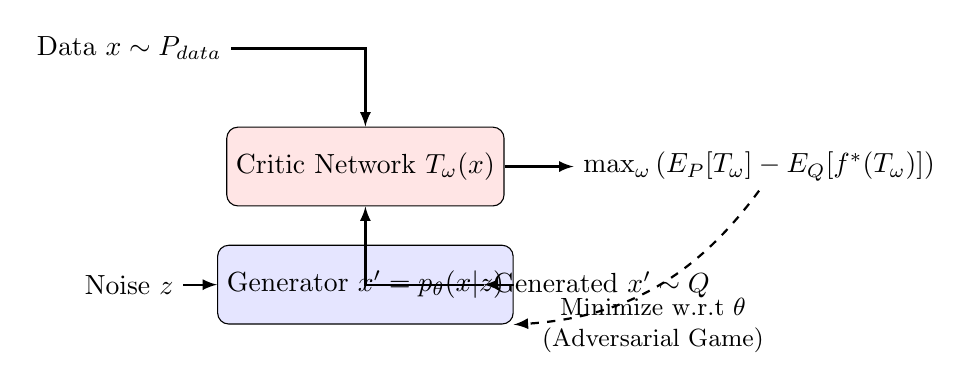
\begin{tikzpicture}[
    box/.style={draw, rounded corners, minimum width=2.5cm, minimum height=1cm, align=center},
    arrow/.style={-latex, thick}
]
    % Nodes
    \node (P) at (0, 3) {Data $x \sim P_{\text{data}}$};
    \node (Z) at (0, 0) {Noise $z$};
    \node[box, fill=blue!10] (G) at (3, 0) {Generator  $x' = p_\theta(x|z)$};
    \node (Q) at (6, 0) {Generated  $x' \sim Q$};
    
    \node[box, fill=red!10] (T) at (3, 1.5) {Critic Network  $T_\omega(x)$};
    
    \node (Obj) at (8, 1.5) {$\max_\omega \left( \mathbb{E}_P[T_\omega] - \mathbb{E}_Q[f^*(T_\omega)] \right)$};

    % Arrows
    \draw[arrow] (Z) -- (G);
    \draw[arrow] (G) -- (Q);
    
    \draw[arrow] (P) -- ++(3,0) -- (T);
    \draw[arrow] (Q) -- ++(-3,0) -- (T);
    
    \draw[arrow] (T) -- (Obj);
    
    % Dashed arrow for generator training
    \draw[arrow, dashed] (Obj.south) to[bend left=25] node[below, align=center, font=\small] {Minimize w.r.t $\theta$\\(Adversarial Game)} (G.south east);
    
\end{tikzpicture}
\caption{The $f$-GAN architecture. A critic network $T_\omega$ is trained to maximize the variational lower bound of the $f$-divergence between the true data distribution $P$ and the generator's distribution $Q$. The generator $p_\theta$ is simultaneously trained to minimize this divergence.}
\label{fig:fgan_arch}
\end{figure}

\subsection{Numerical Example: Deriving the Bound for KL Divergence}
Let's make this concrete by deriving the variational bound for the Kullback-Leibler divergence.
The generator function for KL is $f(u) = u \log u$.
First, we find its Fenchel conjugate $f^*(t)$:
\begin{equation}
    f^*(t) = \sup_{u > 0} \left\{ tu - u \log u \right\}.
\end{equation}
To find the maximum, we take the derivative with respect to $u$ and set it to zero:
\begin{align*}
    \frac{d}{du} (tu - u \log u) &= t - \log u - 1 = 0 \\
    \implies \log u &= t - 1 \\
    \implies u^* &= \exp(t - 1).
\end{align*}
Since the second derivative $-1/u$ is strictly negative for $u>0$, this is a global maximum. Substituting $u^*$ back into the expression yields:
\begin{align*}
    f^*(t) &= t \exp(t-1) - \exp(t-1) \log(\exp(t-1)) \\
           &= t \exp(t-1) - \exp(t-1)(t-1) \\
           &= \exp(t-1).
\end{align*}
Applying Theorem \ref{thm:variational_bound}, the variational bound for KL divergence is:
\begin{equation}
    D_{\text{KL}}(P \parallel Q) = \sup_{T} \left( \mathbb{E}_{x \sim P}[T(x)] - \mathbb{E}_{x \sim Q}[\exp(T(x) - 1)] \right).
\end{equation}
This specific formulation is known as the Nguyen-Wainwright-Jordan (NWJ) bound. 
The optimal critic is $T^*(x) = f'(p(x)/q(x)) = \log(p(x)/q(x)) + 1$. 
If we define a new function $V(x) = T(x) - 1$, the bound becomes the familiar Donsker-Varadhan representation:
\begin{equation}
    D_{\text{KL}}(P \parallel Q) = \sup_{V} \left( \mathbb{E}_{x \sim P}[V(x)] - \mathbb{E}_{x \sim Q}[\exp(V(x)) - 1] \right).
\end{equation}
Notice that the $\log$ is often introduced in practical implementations for numerical stability through Jensen's inequality: $\mathbb{E}[\exp(V(x))] \ge \exp(\mathbb{E}[V(x)])$.

% 3. Horizon Box
\begin{horizon}
While the variational formulation of $f$-divergences provides a mathematically elegant framework for training generative models without explicit densities, it is not without severe practical pathologies. It is conjectured that in high-dimensional spaces, the supports of the true data distribution $P$ and the model distribution $Q$ are often mutually singular---they lie on low-dimensional manifolds that do not perfectly overlap (the Manifold Hypothesis, Chapter 5). 

When $P$ and $Q$ have disjoint supports, the density ratio $p(x)/q(x)$ diverges to infinity or drops to zero. Consequently, most $f$-divergences max out and provide a constant, saturated value. For example, the Jensen-Shannon divergence will quickly saturate to $\log 2$. When the divergence is constant, its gradient with respect to the generator's parameters $\theta$ vanishes. The critic network becomes ``too good'' at distinguishing real from fake data, leaving the generator with no useful learning signal.

An open question is whether one can construct specific $f$-functions that are robust to this dimensional scaling, or if the paradigm inherently fails when supports are disjoint. Future work might show that regularizing the critic's Lipschitz constant implicitly morphs the $f$-divergence into an Integral Probability Metric. Currently, the field has largely shifted toward Wasserstein distances and Optimal Transport (Chapter 24), which naturally handle non-overlapping distributions by measuring the ``cost of moving mass'' rather than relying on point-wise density ratios. Thus, while $f$-divergences are fundamental to information theory, their utility in raw high-dimensional latent spaces may be fundamentally limited.
\end{horizon}

% 4. Summary + Exercises
\section*{Summary}
\begin{itemize}
    \item $f$-divergences provide a generalized family of distance measures between probability distributions, defined by a convex generator function $f$.
    \item Different choices of $f$ lead to well-known divergences like KL, Reverse KL, Jensen-Shannon, and Total Variation, each imposing different behaviors on generative models.
    \item Because computing $f$-divergences directly requires intractable density ratios, we use Fenchel conjugacy to derive a variational lower bound.
    \item This variational bound allows us to estimate the divergence using samples by training a discriminator network $T(x)$, forming the theoretical basis of the $f$-GAN framework.
\end{itemize}

\section*{Exercises}
\begin{enumerate}
    \item \textbf{Deriving the Jensen-Shannon Bound:} Let $f(u) = u \log u - (u+1) \log\left(\frac{u+1}{2}\right)$. Derive the Fenchel conjugate $f^*(t)$ and write out the resulting adversarial objective for estimating the Jensen-Shannon divergence. How does this relate to the original GAN loss proposed by Goodfellow et al. (2014)?
    \item \textbf{Optimal Critic in $\chi^2$ Divergence:} For the Pearson $\chi^2$ divergence where $f(u) = (u-1)^2$, find the Fenchel conjugate $f^*(t)$ and state the variational objective. Show that the optimal critic $T^*(x)$ is exactly $2\left(\frac{p(x)}{q(x)} - 1\right)$. 
    \item \textbf{Vanishing Gradients:} Suppose distributions $P$ and $Q$ are uniform on $[0,1]$ and $[2,3]$ respectively (completely disjoint supports). Compute the KL divergence $D_{\text{KL}}(P \parallel Q)$ and the Jensen-Shannon divergence $D_{\text{JS}}(P \parallel Q)$. What would the gradient of these divergences be if $Q$ was parameterized by a mean $\mu$ (currently at $\mu=2.5$)? Explain why this motivates Wasserstein distances.
\end{enumerate}

% TODO-CITE: Ensure all named results are cited.
